%!TEX root = GeoTopo.tex
%%%%%%%%%%%%%%%%%%%%%%%%%%%%%%%%%%%%%%%%%%%%%%%%%%%%%%%%%%%%%%%%%%%%%
% Henriekes Mitschrieb vom 07.11.2013                               %
%%%%%%%%%%%%%%%%%%%%%%%%%%%%%%%%%%%%%%%%%%%%%%%%%%%%%%%%%%%%%%%%%%%%%
\chapter{Mannigfaltigkeiten und Simplizialkomplexe}
\section{Topologische Mannigfaltigkeiten}
\begin{definition}%
    Sei $(X, \fT)$ ein topologischer Raum und $n \in \mdn$.
    \begin{defenum}
        \item Eine $n$-dimensionale \textbf{Karte}\xindex{Karte} auf
              $X$ ist ein Paar $(U, \varphi)$, wobei $U \in \fT$
              und $\varphi: U \rightarrow V$ Homöomorphismus
              von $U$ auf eine offene Teilmenge $V \subseteq \mdr^n$.
        \item Ein $n$-dimensionaler \textbf{Atlas}\xindex{Atlas} $\atlas$ auf $X$ ist eine
              Familie $(U_i, \varphi_i)_{i \in I}$ von Karten auf $X$,
              sodass $\bigcup_{i \in I} U_i = X$.
        \item $X$ heißt (topologische) $n$-dimensionale \textbf{Mannigfaltigkeit}\xindex{Mannigfaltigkeit},
              wenn $X$ hausdorffsch ist, eine abzählbare Basis der 
              Topologie hat und ein $n$-dimensionalen Atlas besitzt.
    \end{defenum}
\end{definition}

Anschaulich ist also ein $n$-dimensionale Mannigfaltigkeit lokal dem $\mdr^n$ ähnlich.

\begin{bemerkung}
    \begin{bemenum}
        \item Es gibt surjektive, stetige Abbildungen $[0,1] \rightarrow [0,1] \times [0,1]$
        \item Für $n \neq m$ sind $\mdr^n$ und $\mdr^m$ nicht homöomorph.
              Zum Beweis benutzt man den \enquote{Satz von der Gebietstreue} (Brouwer):

              Ist $U \subseteq \mdr^n$ offen und $f: U \rightarrow \mdr^n$
              stetig und injektiv, so ist $f(U)$ offen.

              Ist $n < m$ und $\mdr^m$ homöomorph zu $\mdr^n$, so wäre
              \[f:\mdr^n \rightarrow \mdr^m \rightarrow \mdr^n, \;\;\; (x_1, \dots, x_n) \mapsto (x_1, x_2, \dots, x_n, 0, \dots, 0)\]
              eine stetige injektive Abbildung. Also müsste $f(\mdr^n)$
              offen sein $\Rightarrow$ Widerspruch
    \end{bemenum}
\end{bemerkung}

\begin{beispiel}[Mannigfaltigkeiten]
    \begin{bspenum}
        \item Jede offene Teilmenge $U \subseteq \mdr^n$ ist eine 
              $n$-dimensionale Mannigfaltigkeit mit einem Atlas aus 
              einer Karte.
        \item $\mdc^n$ ist eine $2n$-dimensionale Mannigfaltigkeit
              mit einem Atlas aus einer Karte:
              \[(z_1, \dots, z_n) \mapsto (\Re(z_1), \Im(z_1), \dots, \Re(z_n), \Im(z_n))\]
        \item \xindex{Raum!projektiver}$\praum^n(\mdr) = (\mdr^{n+1} \setminus \Set{0})/_\sim = S^n /_\sim$ und $\praum^n(\mdc)$ sind Mannigfaltigkeiten
              der Dimension $n$ bzw. $2n$, da gilt:

              Sei $U_i := \Set{(x_0: \dots : x_n) \in \praum^n(\mdr) | x_i \neq 0}\;\forall i \in 0, \dots, n$.
              Dann ist $\praum^n(\mdr) = \bigcup_{i=0}^n U_i$ und die Abbildung
              \begin{align*}
                U_i &\rightarrow \mdr^n\\
                (x_0 : \dots : x_n) &\mapsto \left (\frac{x_0}{x_i}, \dots, \frac{x_i}{x_i}, \dots, \frac{x_n}{x_i} \right )\\
                (y_1 : \dots : y_{i-1} : 1 : y_i : \dots : y_n) &\mapsfrom (y_1, \dots, y_n)
              \end{align*}
              ist bijektiv.
              \todo[inline]{Was wird im Folgenden gemacht?}
              Die $U_i$ mit $i = 0, \dots, n$ bilden einen $n$-dimensionalen Atlas:
              \begin{align*}
                      x &= (1:0:0) \in U_0 \rightarrow \mdr^2 & x &\mapsto (0,0)\\
                      y &= (0:1:1) \in U_2 \rightarrow \mdr^2 & y &\mapsto (0,1)
              \end{align*}
              $\text{Umgebung: } \fB_1 (0,1) \rightarrow \Set{(1:u:v) | \|(u,v)\| < 1} = V_1$\\
              $\text{Umgebung: } \fB_1 (0,1) \rightarrow \Set{(w:z:1) | w^2 + z^2 < 1} = V_2$\\

              $V_1 \cap V_2 = \emptyset$?

              $(a:b:c) \in V_1 \cap V_2$\\
              $\Rightarrow a \neq 0$ und $(\frac{b}{a})^2 + (\frac{c}{a})^2 < 1 \Rightarrow \frac{c}{a} < 1$\\
              $\Rightarrow c \neq 0$ und $(\frac{a}{c})^2 + (\frac{b}{c})^2 < 1 \Rightarrow \frac{a}{c} < 1$\\
              $\Rightarrow$ Widerspruch
        \item $S^n = \Set{x \in \mdr^{n+1} | \|x\| = 1}$ ist $n$-dimensionale
              Mannigfaltigkeit.

              Karten: \\
              $D_i := \{(x_1, \dots, x_{n+1}) \in S^n | x_i > 0\} \rightarrow \fB_1 (\underbrace{0, \dots, 0}_{\in \mdr^n})$\\
              $C_i := \{(x_1, \dots, x_{n+1}) \in S^n | x_i < 0\}$\\
              $(x_1, \dots, x_{n+1}) \mapsto (x_1, \dots, \cancel{x_i}, \dots, x_{n+1})$\footnote{$x_i$ wird rausgenommen}\\
              $(x_1, \dots, x_{n}) \mapsto (x_1, \dots, x_{i-1}, \sqrt{1-\sum_{k=1}^n x_k^2}, x_i, \dots, x_n)$, oder $-\sqrt{1-\sum_{k=1}^n x_k^2}$ für $C_i$\\
              $S^n = \bigcup_{i=1}^{n+1} (C_i \cup D_i)$
        \item $[0,1]$ ist keine Mannigfaltigkeit, denn:\\
              Es gibt keine Umgebung von $0$ in $[0,1]$, die homöomorph
              zu einem offenem Intervall ist.
        \item $V_1 = \Set{(x,y) \in \mdr^2 | x \cdot y = 0}$ ist
              keine Mannigfaltigkeit. 

              Das Problem ist $(0,0)$. Wenn man diesen Punkt entfernt,
              zerfällt der Raum in 4 Zusammenhangskomponenten.
              Jeder $\mdr^n$ zerfällt jedoch in höchstens zwei
              Zusammenhangskomponenten, wenn man einen Punkt entfernt.
        \item $V_2 = \Set{(x,y) \in \mdr^2 | x^3 = y^2}$ ist eine
              Mannigfaltigkeit.
        \item $X = (\mdr \setminus \Set{0}) \cup (0_1, 0_2)$ \label{bsp:mannigfaltigkeit8}

              \[U \subseteq X \text{ offen } \gdw 
                \begin{cases}
                    U \text{ offen in } \mdr \setminus \Set{0}, &\text{falls } 0_1 \notin U, 0_2 \in U\\
                    \exists \varepsilon > 0: (-\varepsilon, \varepsilon) \subseteq U &\text{falls } 0_1 \in U, 0_2 \in U
                \end{cases}\]
              Insbesondere sind $(\mdr \setminus \Set{0}) \cup \Set{0_1}$
              und $(\mdr \setminus \Set{0}) \cup \Set{0_2}$ offen und
              homöomorph zu $\mdr$.

              \underline{Aber:} $X$ ist nicht hausdorffsch!
              Denn es gibt keine disjunkten Umgebungen von $0_1$ und
              $0_2$.
        \item \label{bsp:gln-ist-mf}\xindex{Gruppe!allgemeine lineare}$\GL_n(\mdr)$ ist eine Mannigfaltigkeit der Dimension 
              $n^2$, weil offene Teilmengen von $\mdr^{n^2}$ eine
              Mannigfaltigkeit bilden.
    \end{bspenum}
\end{beispiel}

%%%%%%%%%%%%%%%%%%%%%%%%%%%%%%%%%%%%%%%%%%%%%%%%%%%%%%%%%%%%%%%%%%%%%
% Mitschrieb vom 14.11.2013                                         %
%%%%%%%%%%%%%%%%%%%%%%%%%%%%%%%%%%%%%%%%%%%%%%%%%%%%%%%%%%%%%%%%%%%%%
\begin{definition}\xindex{Verklebung}%
    Seien $X, Y$ $n$-dimensionale Mannigfaltigkeiten, $U \subseteq X$
    und $V \subseteq Y$ offen, $\Phi: U \rightarrow V$ ein Homöomorphismus
    $Z = (X \dcup Y) /_\sim$ mit der von $u \sim \Phi(u)\;\forall{u \in U}$
    erzeugten Äquivalenzrelation und der von $\sim$ induzierten 
    Quotiententopologie.

    $Z$ heißt \textbf{Verklebung} von $X$ und $Y$ längs $U$ und $V$.
    $Z$ besitzt einen Atlas aus $n$-dimensionalen Karten.
    Falls $Z$ hausdorffsch ist, ist $Z$ eine $n$-dimensionale 
    Mannigfaltigkeit.
\end{definition}

\begin{bemerkung}
    Sind $X, Y$ Mannigfaltigkeiten der Dimension $n$ bzw. $m$, so ist
    $X \times Y$ eine Mannigfaltigkeit der Dimension $n+m$.
\end{bemerkung}

\begin{beweis}
    Produkte von Karten sind Karten. $\qed$
\end{beweis}

\begin{beispiel}
    Mannigfaltigkeiten mit Dimension 1:
    \begin{enumerate}[label=\arabic*)]
        \item Offene Intervalle, $\mdr$, $(0,1)$ sind alle homöomorph
        \item $S^1$
    \end{enumerate}

    Mannigfaltigkeiten mit Dimension 2:
    \begin{enumerate}[label=\arabic*)]
        \item $\mdr^2$
        \item $S^2$ (0 Henkel)
        \item $T^2$ (1 Henkel)
        \item oder mehr Henkel, wie z.B. der Zweifachtorus in \cref{fig:double-torus}
    \end{enumerate}

    \begin{figure}[htp]
        \centering
        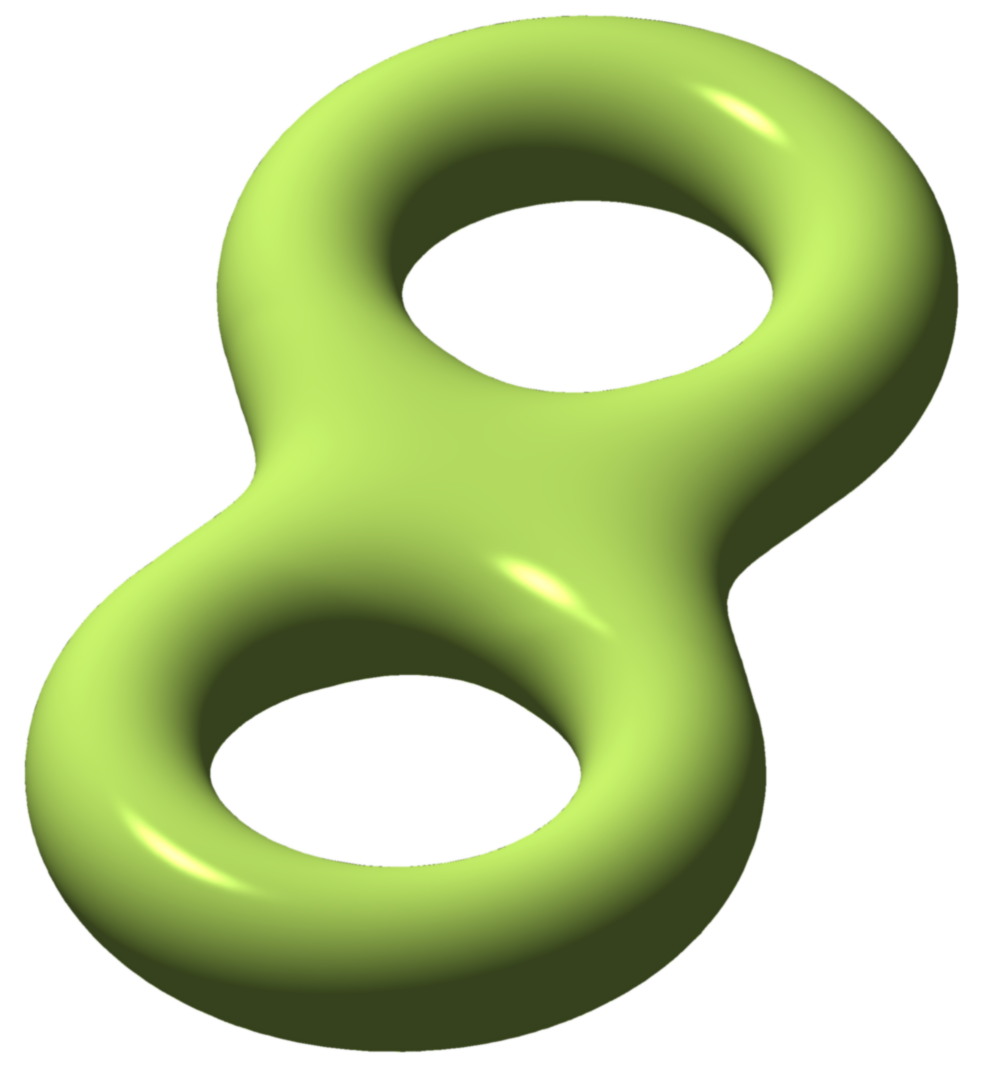
\includegraphics[width=0.2\linewidth, keepaspectratio]{figures/Double-torus-illustration.png}
        \caption{Zweifachtorus}
        \label{fig:double-torus}
    \end{figure}
\end{beispiel}

\begin{bemerkung}
    Sei $n \in \mdn, F:\mdr^n \rightarrow \mdr$ stetig differenzierbar
    und $X = V(F) := \Set{x \in \mdr^n | F(x) = 0}$ das \enquote{vanishing set}\xindex{vanishing set}.

    Dann gilt:
    \begin{bemenum}
        \item $X$ ist abgeschlossen in $\mdr^n$
        \item Ist $\grad(F)(X) \neq 0 \;\;\;\forall{x \in X}$, so ist
              $X$ eine Mannigfaltigkeit der Dimension $n-1$.  \label{bem:Mannigfaltigkeitskriterium}
    \end{bemenum}
\end{bemerkung}

\begin{beweis}\leavevmode
    \begin{enumerate}[label=\alph*),ref=\thedefinition.\alph*]
        \item Sei $y \in \mdr^n \setminus V(F)$. Weil $F$ stetig ist,
              gibt es $\delta > 0$, sodass $F(\fB_\delta(y)) \subseteq \fB_\varepsilon(F(y))$
              mit $\varepsilon = \frac{1}{2} \|F(y)\|$. Folgt
              $\fB_\delta(y) \cap V(F) = \emptyset \Rightarrow \mdr^n \setminus V(F)$
              ist offen.
        \item Sei $x \in X$ mit $\grad(F)(x) \neq 0$, also
              \obda $\frac{\partial F}{\partial X_1} (x) \neq 0$,
              $x = (x_1, \dots, x_n)$, $x' := (x_2, \dots, x_n) \in \mdr^{n-1}$.
              Der Satz von der impliziten Funktion liefert nun:
              Es gibt Umgebungen $U$ von $x'$ und differenzierbare
              Funktionen $g: U \rightarrow \mdr$, sodass
              $G: U \rightarrow \mdr^n, \; u \mapsto (g(u), u)$
              eine stetige Abbildung auf eine offene Umgebung $V$ von
              $x$ in $X$ ist.
    \end{enumerate}  
    $\qed$
\end{beweis}

\begin{beispiel}\xindex{Neilsche Parabel}%
    \begin{bspenum}
        \item $F: \mdr^3 \rightarrow \mdr,\;\;\; (x, y, z) \mapsto x^2 + y^2 + z^2 - 1$,
              $V(F) = S^2$, $\grad(F) = (2x, 2y, 2z) \xRightarrow{\crefabbr{bem:Mannigfaltigkeitskriterium}} S^n$
              ist $n$-dimensionale Mannigfaltigkeit in $\mdr^{n+1}$
        \item $F: \mdr^2 \rightarrow \mdr, \;\;\; (x,y) \mapsto y^2 - x^3$
            \begin{figure}[ht]
                \centering
                \subfloat[$F(x,y) = y^2 - x^3$]{
                    \resizebox{0.45\linewidth}{!}{\documentclass{article}
\usepackage[pdftex,active,tightpage]{preview}
\setlength\PreviewBorder{2mm}
\usepackage{pgfplots}
\pgfplotsset{compat=1.9}

\begin{document}
\begin{preview}
\pgfplotsset{
    colormap={whitered}{
        color(0cm)=(white);
        color(1cm)=(orange!75!red)
    }
}
\begin{tikzpicture}[scale=0.5]
    \begin{axis}[
    colormap name=whitered,
    width=6cm,
    view={155}{45},
    enlargelimits=false,
    grid=major,
    domain=-5:5,
    y domain=-5:5,
    samples=56, %57 : TeX capacity exceeded, sorry [main memory size=3000000].
                % see also http://tex.stackexchange.com/a/7954/5645
    xlabel=$x$,
    ylabel=$y$,
    zlabel={$z$},
    colorbar,
    colorbar style={
        at={(-0.1,0)},
        anchor=south west,
        height=0.25*\pgfkeysvalueof{/pgfplots/parent axis height},
        title={$f(x,y)$}
    }
    ]
      \addplot3[surf] {y*y-x*x*x};
    \end{axis} 
\end{tikzpicture}
\end{preview}
\end{document}
}
                    \label{fig:semicubical-parabola-2d}
                }%
                \subfloat[$y^2 - ax^3 = 0$]{
                    \resizebox{0.45\linewidth}{!}{\documentclass[varwidth=true, border=2pt]{standalone}

\usepackage{pgfplots}
\usepackage{tikz}

\begin{document}
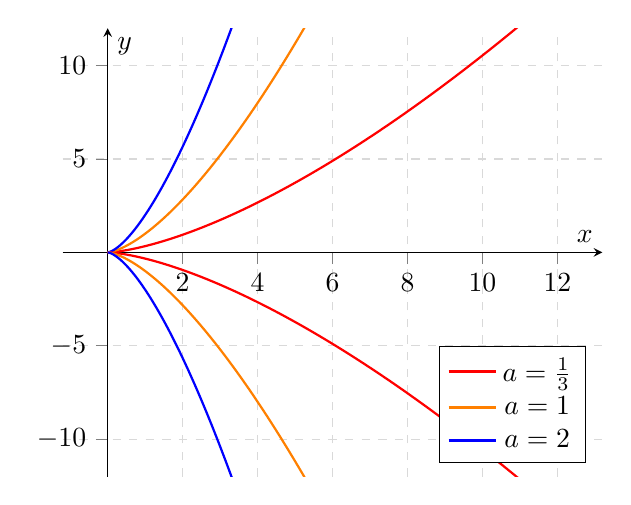
\begin{tikzpicture}
    \begin{axis}[
        legend pos=south east,
        axis x line=middle,
        axis y line=middle,
        grid = major,
        %width=9cm,
        %height=4.5cm,
        grid style={dashed, gray!30},
        xmin= 0,     % start the diagram at this x-coordinate
        xmax= 12,    % end   the diagram at this x-coordinate
        ymin=-10,     % start the diagram at this y-coordinate
        ymax= 10,   % end   the diagram at this y-coordinate
        %axis background/.style={fill=white},
        xlabel=$x$,
        ylabel=$y$,
        %xticklabels={-2,-1.6,...,7},
        tick align=outside,
        %minor tick num=-3,
        enlargelimits=true]
      \addplot[domain=0:12, red, thick,samples=500] {1/3*x^1.5}; 
      \addplot[domain=0:12, orange, thick,samples=500] {1*x^1.5}; 
      \addplot[domain=0:12, blue, thick,samples=500] {2*x^1.5}; 

      \addplot[domain=0:12, red, thick,samples=500] {-1/3*x^1.5}; 
      \addplot[domain=0:12, orange, thick,samples=500] {-1*x^1.5}; 
      \addplot[domain=0:12, blue, thick,samples=500] {-2*x^1.5}; 
      \addlegendentry{$a=\frac{1}{3}$}
      \addlegendentry{$a=1$}
      \addlegendentry{$a=2$}
    \end{axis} 
\end{tikzpicture}
\end{document}
}
                    \label{fig:semicubical-parabola-3d}
                }%
                \label{Neilsche-Parabel}
                \caption{Rechts ist die Neilsche Parabel für verschiedene Parameter $a$.}
            \end{figure}
              Es gilt: $\grad(F) = (-3x^2, 2y)$. Also: $\grad(0,0) = (0,0)$.
              Daher ist \cref{bem:Mannigfaltigkeitskriterium}
              nicht anwendbar, aber $V(F)$ ist trotzdem
              eine 1-dimensionale topologische Mannigfaltigkeit.
    \end{bspenum}
\end{beispiel}

\begin{definition}\xindex{Mannigfaltigkeit!mit Rand}%
    Sei $X$ ein Hausdorffraum mit abzählbarer Basis der Topologie.
    $X$ heißt $n$-dimensionale \textbf{Mannigfaltigkeit mit Rand},
    wenn es einen Atlas $(U_i, \varphi_i)$ gibt, wobei $U_i \subseteq X_i$
    offen und $\varphi_i$ ein Homöomorphismus auf eine offene 
    Teilmenge von 
    \[R_{+,0}^n := \Set{(x_1, \dots, x_n) \in \mdr^n | x_m \geq 0}\]
    ist.
\end{definition}

$R_{+,0}^n$ ist ein \enquote{Halbraum}\xindex{Halbraum}.

\begin{figure}[ht]
    \centering
    \subfloat[Halbraum]{
        \begin{tikzpicture}
    \draw [white,step=0.5cm, pattern=north east lines] (0,0) rectangle (2,1);
    \draw[very thick] (0,0) -- (2,0);

    \node at (2.4,0.5) {$\stackrel{\sim}{=}$};

\begin{scope}[shift={(4,0)}]
    \draw[white,pattern=north east lines] ([shift={(180:1cm)}]-0.0,0) arc (180:0:1cm);
    \draw[very thick] (-1,0) -- (1,0);
\end{scope}
\end{tikzpicture}

        \label{fig:half-space}
    }%

    \subfloat[Pair of pants]{
        \resizebox{0.45\linewidth}{!}{\begin{tikzpicture}[tqft/flow=east]
    \node[tqft/pair of pants,draw,rotate=-180] (a) {};
    \draw (-1.02,-1) ellipse (0.2cm and 0.35cm);
    \draw (-1.02,+1) ellipse (0.2cm and 0.35cm);
    \draw[dashed] (1,0) ellipse (0.175cm and 0.35cm);

    \draw (2.3,0) ellipse (0.7cm and 1.5cm);
    \draw (2.3,+0.5) circle (0.3cm);
    \draw (2.3,-0.5) circle (0.3cm);

    \node at (1.38,0) {$\stackrel{\sim}{=}$};
\end{tikzpicture}
}
        \label{fig:pair-of-pants}
    }%
    \subfloat[Sphäre mit einem Loch]{
        \resizebox{0.45\linewidth}{!}{\begin{tikzpicture}[tqft/flow=east]
    \draw (0,0) circle (2cm);
    \draw (0,0) ellipse (2cm and 0.35cm);
    \draw[white,fill=white] (0,0.1) ellipse (1.95cm and 0.35cm);
    \draw[dashed] (0,0) ellipse (2cm and 0.35cm);

    \begin{scope}[rotate=45]
        \draw (0.5,1.2) ellipse (0.5cm and 0.4cm);
    \end{scope}

    \node at (2.38,0) {$\stackrel{\sim}{=}$};

    \draw (3.8,0) circle (1cm);
\end{tikzpicture}
}
        \label{fig:sphere-with-hole}
    }%
    \label{Mannigfaltigkeiten mit Rand}
    \caption{Beispiele für Mannigfaltigkeiten mit Rand}
\end{figure}

\begin{definition}\xindex{Rand}%
    Sei $X$ eine $n$-dimensionale Mannigfaltigkeit mit Rand und
    Atlas $\atlas$. Dann heißt 
    \[\partial X := \bigcup_{(U, \varphi) \in \atlas} \Set{x \in U | \varphi (x) = 0}\]
    \textbf{Rand} von $X$.
\end{definition}

$\partial X$ ist eine Mannigfaltigkeit der Dimension $n-1$.

\begin{definition}\xindex{Kartenwechsel}\index{Uebergangsfunktion@""Ubergangsfunktion|see{Kartenwechsel}}%
    Sei $X$ eine $n$-dimensionale Mannigfaltigkeit mit Atlas
    $(U_i, \varphi_i)_{i \in I}$

    Für $i, j \in I$ mit $U_i, U_j \neq \emptyset$ heißt
              \begin{align*}
                \varphi_{ij} &:= \varphi_j \circ \varphi_i^{-1}\\
                \varphi_i (U_i \cap U_j) &\rightarrow \varphi_j (U_i \cap U_j)
              \end{align*}
              \textbf{Kartenwechsel} oder \textbf{Übergangsfunktion}.
\end{definition}

\begin{figure}[htp]
    \centering
    \documentclass[varwidth=true, border=2pt]{standalone}
\usepackage{amsmath,amssymb}% math symbols / fonts
\usepackage{tikz}
\usepackage{tqft}
\usetikzlibrary{patterns}

\begin{document}
    \begin{tikzpicture}[tqft/flow=east]
        \draw (0,0) ellipse (2cm and 1cm);
        \draw (0,-2) ellipse (3cm and 0.8cm);
        \def\ringa{(-0.3,0) circle (0.5cm)}
        \def\ringb{(+0.3,0) circle (0.5cm)}

        \begin{scope}[even odd rule]
            \clip \ringa;
            \fill[pattern color=red,pattern=north east lines] \ringb;
        \end{scope}

        \begin{scope}[even odd rule,shift={(-0.7,-2)}]
            \clip \ringa;
            \fill[draw=red,pattern color=red,pattern=north east lines] \ringb;
        \end{scope}

        \begin{scope}[even odd rule,shift={(+0.7,-2)}]
            \clip \ringb;
            \fill[draw=red,pattern color=red,pattern=north east lines] \ringa;
        \end{scope}
        \draw \ringa;
        \draw \ringb;

        \node at (-1,0.3) {$U_i$};
        \node at (+1,0.3) {$U_j$};
        \node at (-1.9,-2) {$V_i$};
        \node at (+1.9,-2) {$V_j$};
        \node at (+2.0,0.7) {$X$};
        \node at (+2.4,-1.3) {$\mathbb{R}^n$};


        \path[->] (-0.35,0)  edge [bend angle=10,bend right] node[label={[label distance=0.1cm]210:$\varphi_i$}] {} (-1,-1.5);
        \path[->] (+0.35,0)  edge [bend angle=10,bend left]  node[label={[label distance=0.1cm]-30:$\varphi_j$}] {} (+1,-1.5);

        \draw (-1,-2) circle (0.5cm);
        \draw (+1,-2) circle (0.5cm);

        \draw[->, red, thick] (-0.3,-2) -- (0.3,-2);
    \end{tikzpicture}
\end{document}

    \caption{Kartenwechsel}
    \label{fig:kartenwechsel}
\end{figure}

%%%%%%%%%%%%%%%%%%%%%%%%%%%%%%%%%%%%%%%%%%%%%%%%%%%%%%%%%%%%%%%%%%%%%
% Mitschrieb vom 19.11.2013                                         %
%%%%%%%%%%%%%%%%%%%%%%%%%%%%%%%%%%%%%%%%%%%%%%%%%%%%%%%%%%%%%%%%%%%%%
\section{Differenzierbare Mannigfaltigkeiten}\label{sec:8}
\begin{definition}%
    Sei $X$ eine $n$-dimensionale Mannigfaltigkeit mit Atlas $(U_i, \varphi_i)_{i \in I}$.

    \begin{defenum}
        \item $X$ heißt \textbf{differenzierbare Mannigfaltigkeit der Klasse $C^k$}\xindex{Mannigfaltigkeit!differenzierbare},
              wenn jede Kartenwechselabbildung $\varphi_{ij},\;i,j \in I$
              $k$-mal stetig differenzierbar ist.
        \item $X$ heißt \textbf{differenzierbare Mannigfaltigkeit}\xindex{Mannigfaltigkeit!glatte},
              wenn $X$ eine differenzierbare Mannigfaltigkeit der
              Klasse $C^\infty$ ist.
    \end{defenum}
\end{definition}

Differenzierbare Mannigfaltigkeiten der Klasse $C^\infty$ werden auch
\textit{glatt} genannt.

\begin{definition}%
    Sei $X$ eine differenzierbare Mannigfaltigkeit der Klasse $C^k$ 
    ($k \in \mdn \cup \Set{\infty}$) mit Atlas $\atlas = (U_i, \varphi_i)_{i \in I}$.

    \begin{defenum}
        \item Eine Karte $(U, \varphi)$ auf $X$ heißt \textbf{verträglich}\xindex{verträglich}
              mit $\atlas$, wenn alle Kartenwechsel $\varphi \circ \varphi_i^{-1}$
              und $\varphi_i \circ \varphi^{-1}$ ($i \in I$ mit $U_i \cap U \neq \emptyset$)
              differenzierbar von Klasse $C^k$ sind.
        \item Die Menge aller mit $\atlas$ verträglichen Karten auf 
              $X$ bildet einen maximalen Atlas der Klasse $C^k$. Er
              heißt \textbf{$C^k$-Struktur}\xindex{Ck-Struktur@$C^k$-Struktur} auf $X$.
            
              Eine $C^\infty$-Struktur heißt auch \textbf{differenzierbare Struktur}\xindex{Struktur!differenzierbare}
              auf $X$.
    \end{defenum}
\end{definition}

\begin{bemerkung}
    Für $n \geq 4$ gibt es auf $S^n$ mehrere verschiedene differenzierbare
    Strukturen, die sogenannten \enquote{exotische Sphären}\xindex{Sphäre!exotische}.
\end{bemerkung}

\begin{definition}
    Seien $X, Y$ differenzierbare Mannigfaltigkeiten der Dimension
    $n$ bzw. $m$, $x \in X$.

    \begin{defenum}
        \item Eine stetige Abbildung $f:X \rightarrow Y$ heißt\label{def:stetigeAbbildungDiffbar}
              \textbf{differenzierbar}\xindex{Abbildung!differenzierbare}
              in $x$ (von Klasse $C^k$),
              wenn es Karten $(U, \varphi)$ von $X$ mit
              $x \in U$ und $(V, \psi)$ von $Y$ mit $f(U) \subseteq V$
              gibt, sodass $\psi \circ f \circ \varphi^{-1}$ stetig
              differenzierbar von Klasse $C^k$ in $\varphi(x)$ ist.
        \item $f$ heißt \textbf{differenzierbar}
              (von Klasse $C^k$), wenn $f$ in jedem $x \in X$ 
              differenzierbar ist.
        \item $f$ heißt \textbf{Diffeomorphismus}\xindex{Diffeomorphismus},
              wenn $f$ differenzierbar von Klasse $C^\infty$ ist und
              es eine differenzierbare Abbildung $g: Y \rightarrow X$
              von Klasse $C^\infty$ gibt mit $g \circ f = \id_X$
              und $f \circ g = \id_Y$.
    \end{defenum}
\end{definition}

\begin{bemerkung}
    Die Bedingung in \cref{def:stetigeAbbildungDiffbar} hängt nicht
    von den gewählten Karten ab.
\end{bemerkung}

\begin{beweis}
    Seien $(U', \varphi')$ und $(V', \psi')$ Karten von $X$ bzw. $Y$
    um $x$ bzw. $f(x)$ mit $f(U') \subseteq V'$.
    
    $\Rightarrow \psi' \circ f \circ (\varphi')^{-1}$\\
    $= \psi' \circ ( \psi^{-1} \circ \psi) \circ f \circ (\varphi^{-1} \circ \varphi ) \circ (\varphi')^{-1}$

    ist genau dann differenzierbar, wenn $\psi \circ f \circ \varphi^{-1}$
    differenzierbar ist.
\end{beweis}

\begin{beispiel}
    $f: \mdr \rightarrow \mdr, \;\;\; x \mapsto x^3$ ist kein
    Diffeomorphismus, aber Homöomorphismus, da mit $g(x) := \sqrt[3]{x}$
    gilt: $f \circ g = \id_\mdr, \;\;\; g \circ f = \id_\text{\mdr}$
\end{beispiel}

\begin{bemerkung}
    Sei $X$ eine glatte Mannigfaltigkeit. Dann ist
    \[\Diffeo(X) := \Set{f:X \rightarrow X | f \text{ ist Diffeomorphismus}}\]
    eine Untergruppe von $\Homoo(X)$.
\end{bemerkung}

\begin{definition}\label{def:8.5}\xindex{Fläche!reguläre}\xindex{Parametrisierung!reguläre}%
    $S \subseteq \mdr^3$ heißt \textbf{reguläre Fläche} $:\gdw$
    $\forall s \in S\;\exists $ Umgebung $V(s) \subseteq \mdr^3$ $\exists U \subseteq \mdr^2$ offen: 
    $\exists \text{ differenzierbare Abbildung } F: U \rightarrow V \cap S$: 
    $\text{Rg}(J_F(u)) = 2\;\;\;\forall u \in U$.

    $F$ heißt (lokale) \textbf{reguläre Parametrisierung} von $S$.

    \begin{align*}
        F(u,v) &= \left (x(u,v), y(u,v), z(u,v) \right )\\
        J_F(u,v) &= \begin{pmatrix}
            \frac{\partial x}{\partial u} (p) & \frac{\partial x}{\partial v} (p)\\
            \frac{\partial y}{\partial u} (p) & \frac{\partial y}{\partial v} (p)\\
            \frac{\partial z}{\partial u} (p) & \frac{\partial z}{\partial v} (p)
        \end{pmatrix}
    \end{align*}
\end{definition}

\begin{beispiel}
    \begin{bspenum}
        \item Rotationsflächen: Sei $r:\mdr \rightarrow \mdr_{> 0}$
              eine differenzierbare Funktion.

              $F: \mdr^2 \rightarrow \mdr^3 \;\;\; (u,v) \mapsto (r(u) \cos (u), r(v) \sin(u), v)$


            \begin{figure}[htp]
                \centering
                \subfloat[Kugelkoordinaten]{
                    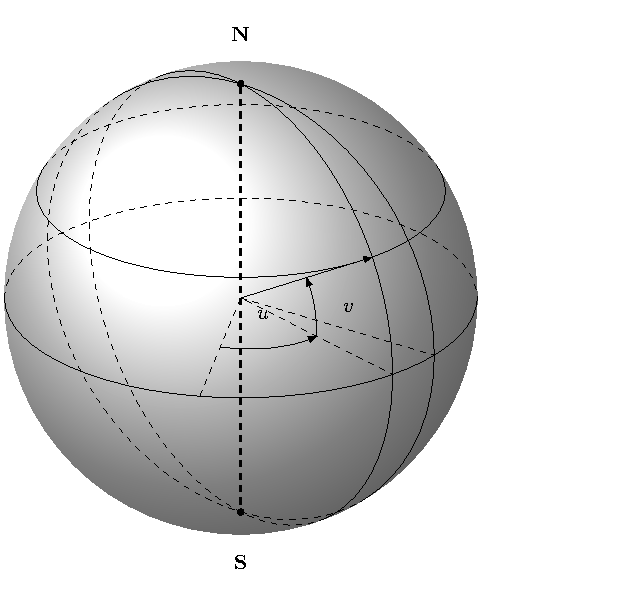
\includegraphics[width=0.45\linewidth, keepaspectratio]{figures/spherical-coordinates.pdf}
                    \label{fig:spherical-coordinates}
                }%
                \subfloat[Rotationskörper]{
                    \resizebox{0.45\linewidth}{!}{% Author: Marco Miani
\documentclass[varwidth=true, border=2pt]{standalone}

\usepackage{pgfplots}
\pgfplotsset{compat=1.9}

\begin{document}
    \pgfplotsset{
        colormap={whitered}{
            color(0cm)=(white);
            color(1cm)=(orange!75!red)
        }
        %colormap={color}{color(0cm)=(white); color(1cm)=(blue)}
    }
    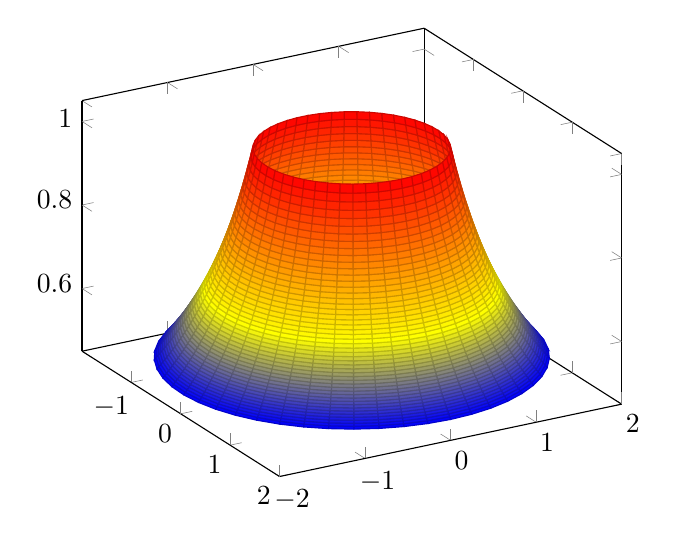
\begin{tikzpicture}
     \begin{axis}[view={60}{30}]
      \addplot3[surf,
      samples=50,
      domain=1:2,y domain=0:2*pi,
      z buffer=sort]
      %({(2 + tan(deg(y)))*cos((deg(x)))}, {(2 + cos(x)) * sin(x)}, {x});
      ({x * cos(deg(y))}, {x * sin(deg(y))}, {1/x});
     \end{axis}
    \end{tikzpicture}
\end{document}
}
                    \label{fig:solid-of-revolution}
                }%

                \subfloat[Sinus und Kosinus haben keine gemeinsame Nullstelle]{
                    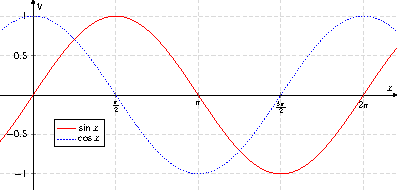
\includegraphics[width=0.8\linewidth, keepaspectratio]{figures/sin-cos.pdf}
                    \label{fig:sin-cos}
                }%
                \label{fig:example-image-gallery-1}
                %\caption{}
            \end{figure}

            \[J_F(u,v) = 
            \begin{pmatrix}
                -r(v) \sin u & r'(v) \cos u\\
                r(v) \cos u  & r'(v) \sin u\\
                 0           & 1
            \end{pmatrix}\]
            hat Rang 2 für alle $(u,v) \in \mdr^2$.
        \item Kugelkoordinaten: $F: \mdr^2 \rightarrow \mdr^3$,\\
              $(u, v) \mapsto (R \cos v \cos u, R \cos v \sin u, R \sin v)$\\
              Es gilt: $F(u,v) \in S_R^2$, denn 
                \begin{align*}
                    & R^2 \cos^2(v) \cos^2(u) + R^2 \cos^2(v) \sin^2(u) + R^2 \sin^2(v)\\
                    =& R^2 (\cos^2(v) \cos^2(u) + \cos^2(v) \sin^2(u) + \sin^2(v))\\
                    =& R^2 \left (\cos^2(v) (\cos^2(u) + \sin^2(u)) + \sin^2(v) \right)\\
                    =& R^2 \left (\cos^2(v) + \sin^2(v) \right)\\
                    =&R^2
                \end{align*}

                Die Jacobi-Matrix
                \[J_F(u,v) = 
                \begin{pmatrix}
                    -R \cos v \sin u & -R \sin v \cos u\\
                    R \cos v \cos u  & -R \sin v \sin u\\
                    0                & R \cos v
                \end{pmatrix}\]
                hat Rang 2 für $\cos v \neq 0$. In $N$ und $S$ ist
                $\cos v = 0$.
    \end{bspenum}
\end{beispiel}

%%%%%%%%%%%%%%%%%%%%%%%%%%%%%%%%%%%%%%%%%%%%%%%%%%%%%%%%%%%%%%%%%%%%%
% Mitschrieb vom 21.11.2013                                         %
%%%%%%%%%%%%%%%%%%%%%%%%%%%%%%%%%%%%%%%%%%%%%%%%%%%%%%%%%%%%%%%%%%%%%
\begin{bemerkung}\label{kor:regular-surface-mannigfaltigkeit}
    Jede reguläre Fläche $S \subseteq \mdr^3$ ist eine 2-dimensionale,
    differenzierbare Mannigfaltigkeit.
\end{bemerkung}

\begin{beweis}\leavevmode

    \todo[inline]{Was ist $F_i$, was $F_j$? Was ist $U_i$, was $U_j$?}

    \underline{z.Z.:} $F_j^{-1} \circ F_i$ ist ein Diffeomorphismus.

    \begin{figure}[htp]
        \centering
        \documentclass[varwidth=true, border=2pt]{standalone}
\usepackage{amsmath,amssymb}% math symbols / fonts
\usepackage{tikz}
\usepackage{tqft}
\usetikzlibrary{patterns}

\begin{document}
    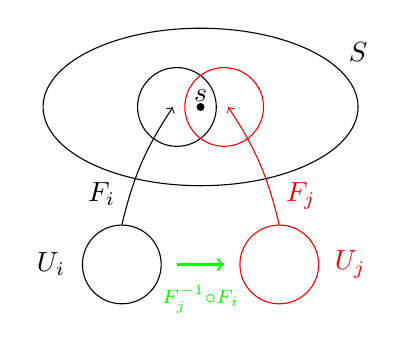
\begin{tikzpicture}
        \tikzstyle{point}=[circle,thick,draw=black,fill=black,inner sep=0pt,minimum width=2pt,minimum height=2pt]
        \draw (0,0) ellipse (2cm and 1cm);
        \def\ringa{(-0.3,0) circle (0.5cm)}
        \def\ringb{(+0.3,0) circle (0.5cm)}

        \draw \ringa;
        \draw[red] \ringb;

        %\node at (-1,0.3) {$U_i$};
        %\node at (+1,0.3) {$U_j$};
        \node at (-1.9,-2) {$U_i$};
        \node[red] at (+1.9,-2) {$U_j$};
        \node at (+2.0,0.7) {$S$};
        \node[point,label={[label distance=-0.1cm]90:$s$}] at (0,0) {};


        \path[<-] (-0.35,0)  edge [bend angle=10,bend right] node[label={[label distance=0.1cm]210:$F_i$}] {} (-1,-1.5);
        \path[<-,red] (+0.35,0)  edge [bend angle=10,bend left]  node[label={[label distance=0.1cm]-30:$F_j$}] {} (+1,-1.5);

        \draw (-1,-2) circle (0.5cm);
        \draw[red] (+1,-2) circle (0.5cm);

        \path[->, green, thick] (-0.3,-2) edge node[label=below:$\scriptstyle F_j^{-1} \circ F_i$] {} (0.3,-2);
    \end{tikzpicture}
\end{document}

        \caption{Reguläre Fläche $S$ zum Beweis von \cref{kor:regular-surface-mannigfaltigkeit}}
        \label{fig:parametric-surface-mapping}
    \end{figure}
    

    \underline{Idee:} Finde differenzierbare Funktion $\widetilde{F_j^{-1}}$
    in Umgebung $W$ von $s$, sodass $\widetilde{F_j^{-1}}|_{S \cap W} = F_j^{-1}$.

    \underline{Ausführung:} Sei $u_0 \in U_i$, $v_0 \in U_j$ mit $F_i(u_0) = s = F_j(v_0)$.

    Da $\rang(J_{F_j}(v_0)) = 2$ ist, ist \obda 
    \[\det 
        \begin{pmatrix}
            \frac{\partial x}{\partial u} & \frac{\partial x}{\partial v}\\
            \frac{\partial y}{\partial u} & \frac{\partial y}{\partial v}
        \end{pmatrix} (v_0) \neq 0
    \]

    und $F_j(u,v) = \left ( x(u,v), y(u,v), z(u,v) \right)$.

    Definiere $\widetilde{F_j}: U_j \times \mdr \rightarrow \mdr^3$ durch
    \[\widetilde{F_j} (u, v, t) := \left(x(u,v), y(u,v), z(u,v)+t \right )\]
    
    Offensichtlich: $\widetilde{F_j} |_{U_j \times \Set{0}} = F_j$

    \[J_{\widetilde{F_j}} = 
    \begin{pmatrix}
        \frac{\partial x}{\partial u}   & \frac{\partial x}{\partial v} & 0\\
        \frac{\partial y}{\partial u}   & \frac{\partial y}{\partial v} & 0\\
        \frac{\partial z}{\partial u}   & \frac{\partial z}{\partial v} & 1
    \end{pmatrix} \Rightarrow \det J_{\widetilde{F_j}} (v_0, 0) \neq  0\]

    $\xRightarrow{\text{Analysis II}}$ Es gibt Umgebungen $W$ von
    $F_j$ von $\widetilde{F_j}(v_0, 0) = F_j(v_0) = s$, sodass $\widetilde{F_j}$
    auf $W$ eine differenzierbar Inverse $F_j^{-1}$ hat.

    Weiter gilt:
    \begin{align*}
        \widetilde{F_j}^{-1}|_{W \cap S} &= F_j^{-1} |_{W \cap S}\\
        \Rightarrow F_j^{-1} \circ F_i |_{F_i^{-1} (W \cap S)} &= F_j^{-1} \circ F_i |_{F_i^{-1} (W \cap S)}
    \end{align*}
    ist differenzierbar.
\end{beweis}

\begin{definition}%
    Sei $G$ eine Mannigfaltigkeit und $(G, \circ)$ eine Gruppe.

    \begin{defenum}
        \item $G$ heißt \textbf{topologische Gruppe}\xindex{Gruppe!topologische},
              wenn die Abbildungen $\circ: G \times G \rightarrow G$
              und $\iota: G \rightarrow G$ definiert durch
              \[g \circ h := g \cdot h \text{ und } \iota(g) := g^{-1}\]
              stetig sind.
        \item Ist $G$ eine differenzierbare Mannigfaltigkeit, so heißt
              $G$ \textbf{Lie-Gruppe}\xindex{Lie-Gruppe}, wenn
              $(G, \circ)$ und $(G, \iota)$ differenzierbar sind.
    \end{defenum}
\end{definition}

\begin{beispiel}[Lie-Gruppen]
    \begin{bspenum}
        \item Alle endlichen Gruppen sind 0-dimensionale Lie-Gruppen.
        \item $\GL_n(\mdr)$ 
              % ist eine Lie-Gruppe, da sie nach \cref{bsp:gln-ist-mf} eine Mannigfaltigkeit ist.
              % $\det: \GL_n \rightarrow \mdr$ ist eine stetige Abbildung.
        \item $(\mdr^\times, \cdot)$
        \item $(\mdr_{>0}, \cdot)$
        \item $(\mdr^n, +)$, denn $A \cdot B (i,j) = \sum_{k=1}^n a_{ik} b_{kj}$ ist
              nach allen Variablen differenzierbar

              $(A^{-1}) (i,j) = \frac{\det(A_{ij})}{\det A}$

              \[A_{ij} = \begin{pmatrix}
                a_{i1} & \dots  & a_{in}\\
                \vdots & \ddots & \vdots\\
                a_{n1} & \dots  & a_{nn}
              \end{pmatrix} \in \mdr^{(n-1) \times (n-1)}\]

            ist differenzierbar.

            $\det A_{ij}$ kann $0$ werden, da:
            \[\begin{pmatrix}1 & 1\\-1&0\end{pmatrix}\]
        \item $\SL_n(\mdr) = \Set{A \in \GL_n(\mdr) | \det(A) = 1}$
    \end{bspenum}
\end{beispiel}

\begin{bemerkung}
    Ist $G$ eine Lie-Gruppe und $g \in G$, so ist die Abbildung
    \begin{align*}
        l_g &: G \rightarrow G\\
        h  &\mapsto g \cdot h
    \end{align*}

    ein Diffeomorphismus.
\end{bemerkung}

\section{Simplizialkomplex}
\begin{definition}\xindex{Lage!allgemeine}%
    Seien $v_0, \dots, v_k \in \mdr^n$ Punkte.\xindex{Punkt}
    \begin{defenum}
        \item $v_0, \dots, v_k$ sind \textbf{in allgemeiner Lage}\\
        \hspace{\labelwidth}\phantom{--}$\gdw$ es gibt keinen $(k-1)$-dimensionalen
              affinen Untervektorraum, der $v_0, \dots, v_k$ enthält\\
        \hspace{\labelwidth}\phantom{--}$\gdw v_1 - v_0, \dots, v_k - v_0$ sind linear unabhängig.
        \item $\conv(v_0, \dots, v_k) := \Set{\sum_{i=0}^k \lambda_i v_i | \lambda_i \geq 0, \sum_{i=0}^k \lambda_i = 1} $
    \end{defenum}
\end{definition}

\begin{definition}
    \begin{defenum}
        \item Sei $\Delta^n = \conv(e_0, \dots, e_n) \subseteq \mdr^{n+1}$
              die konvexe Hülle der Standard-Basisvektoren $e_0, \dots, e_n$.

              Dann heißt $\Delta^n$ \textbf{Standard-Simplex}\xindex{Standard-Simplex}
              und $n$ die Dimension des Simplex.
        \item Für Punkte $v_0, \dots, v_k$ im $\mdr^n$ in allgemeiner
              Lage heißt $\Delta (v_0, \dots, v_k) = \conv(v_0, \dots, v_k)$
              ein \textbf{$k$-Simplex}\xindex{Simplex} in $\mdr^n$.
        \item Ist $\Delta (v_0, \dots, v_k)$ ein $k$-Simplex und
              $I = \Set{i_0, \dots, i_r} \subseteq \Set{0, \dots, k}$,
              so ist $s_{i_0, \dots, i_r} := \conv(v_{i_0}, \dots, v_{i_r})$
              ein $r$-Simplex und heißt
              \textbf{Teilsimplex}\xindex{Teilsimplex} oder \textbf{Seite}\xindex{Seite}
              von $\Delta$.
    \end{defenum}
\end{definition}

\begin{figure}[ht]
    \centering
    \subfloat[0-Simplex $\Delta^0$]{
        \parbox{5cm}{\centering\documentclass[varwidth=true, border=2pt]{standalone}

\usepackage{tikz}
\usepackage{amsmath,amssymb}

\begin{document}
    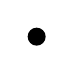
\begin{tikzpicture}[thick]
        \draw[thick, fill=black, black] (0cm,0cm) circle(0.1cm);
        %\node[below] {$1$};
    \end{tikzpicture}
\end{document}
}
        \label{fig:simplex-0}
    }

    \subfloat[1-Simplex $\Delta^1$]{
        \documentclass[varwidth=true, border=2pt]{standalone}

\usepackage{pgfplots}
\usepackage{tikz}
\usepackage{tkz-fct}
\usetikzlibrary{shapes.misc}

\begin{document}
\begin{tikzpicture}
    \tikzstyle{point}=[thick,draw=black,cross out,inner sep=0pt,minimum width=4pt,minimum height=4pt]
    \begin{axis}[
        legend pos=south west,
        axis x line=middle,
        axis y line=middle,
        grid = major,
        width=5cm,
        height=5cm,
        grid style={dashed, gray!30},
        xmin=0,    % start the diagram at this x-coordinate
        xmax=3,    % end   the diagram at this x-coordinate
        ymin=0,    % start the diagram at this y-coordinate
        ymax=3,    % end   the diagram at this y-coordinate
        %xlabel=$x$,
        %ylabel=$y$,
        tick align=outside,
        minor tick num=-3,
        enlargelimits=true,
        tension=0.08]
      \addplot[domain=0:2.5, red, thick,samples=20] {-x+2.5};
      \node[point,label={[label distance=0cm]45:$e_0$}] at (axis cs:2.5,0) {};
      \node[point,label={[label distance=0cm]0:$e_1$}] at (axis cs:0,2.5) {};
    \end{axis} 
\end{tikzpicture}
\end{document}

        \label{fig:simplex-1}
    }%
    \subfloat[2-Simplex $\Delta^2$]{
        \documentclass[varwidth=true, border=2pt]{standalone}

\usepackage{pgfplots}
\usepackage{tikz}
\usepackage{tkz-fct}
\usetikzlibrary{shapes.misc}

\begin{document}
\begin{tikzpicture}
    \tikzstyle{point}=[thick,draw=black,cross out,inner sep=0pt,minimum width=4pt,minimum height=4pt]
    \begin{axis}[
        legend pos=south west,
        axis x line=middle,
        axis y line=middle,
        grid = major,
        width=5cm,
        height=5cm,
        grid style={dashed, gray!30},
        xmin=0,    % start the diagram at this x-coordinate
        xmax=3,    % end   the diagram at this x-coordinate
        ymin=0,    % start the diagram at this y-coordinate
        ymax=3,    % end   the diagram at this y-coordinate
        tick align=outside,
        minor tick num=-3,
        enlargelimits=true,
        tension=0.08]
        \node (a)[point,label={[label distance=0cm]5:$e_0$}] at (axis cs:2.5,0) {};
        \node (b)[point,label={[label distance=0cm]5:$e_1$}] at (axis cs:0,2.5) {};
        \node (c)[point,label={[label distance=0cm]0:$e_2$}] at (axis cs:2,2) {};
        \draw[thick,fill=orange!50] (a.center) -- (b.center) -- (c.center) -- cycle;
    \end{axis} 
\end{tikzpicture}
\end{document}

        \label{fig:simplex-2}
    }%
    \subfloat[3-Simplex $\Delta^3$]{
        \begin{tikzpicture}
    \tikzstyle{point}=[thick,draw=black,cross out,inner sep=0pt,minimum width=4pt,minimum height=4pt]

    \node (a)[point,label={[label distance=0cm]180:$e_0$}] at (0,0) {};
    \node (b)[point,label={[label distance=0cm]0:$e_1$}] at (2,0) {};
    \node (c)[point,label={[label distance=0cm]0:$e_2$}] at (1,2) {};
    \node (d)[point,label={[label distance=0cm]0:$e_3$}] at (1,0.7) {};
    \draw (a.center) -- (b.center) -- (c.center) -- cycle;
    \draw[dashed] (a.center) -- (d.center) -- (b.center);
    \draw[dashed] (d.center) -- (c.center);
\end{tikzpicture}

        \label{fig:simplex-3}
    }%
    \label{fig:k-simplexe}
    \caption{Beispiele für $k$-Simplexe}
\end{figure}


%%%%%%%%%%%%%%%%%%%%%%%%%%%%%%%%%%%%%%%%%%%%%%%%%%%%%%%%%%%%%%%%%%%%%
% Mitschrieb vom 21.11.2013                                         %
%%%%%%%%%%%%%%%%%%%%%%%%%%%%%%%%%%%%%%%%%%%%%%%%%%%%%%%%%%%%%%%%%%%%%
\begin{definition}%
    \begin{enumerate}[label=\alph*),ref=\thedefinition.\alph*]
        \item Eine endliche Menge $K$ von Simplizes im $\mdr^n$
              heißt (endlicher) \textbf{Simplizialkomplex}\xindex{Simplizialkomplex},
              wenn gilt:
            \begin{enumerate}[label=(\roman*),ref=\theenumii.\roman*]
                \item Für $\Delta \in K$ und $S \subseteq \Delta$ Teilsimplex
                      ist $S \in K$.
                \item \label{def:simplizialkomplex.ii} Für $\Delta_1, \Delta_2 \in K$ ist 
                      $\Delta_1 \cap \Delta_2$ leer oder ein 
                        Teilsimplex von $\Delta_1$ und von 
                      $\Delta_2$. 
            \end{enumerate}
        \item $|K| := \bigcup_{\Delta \in K} \Delta$ (mit Teilraumtopologie)
              heißt \textbf{geometrische Realisierung}\xindex{Realisierung!geometrische}
              von $K$.
        \item Ist $d = \max \Set{ k \in \mdn | K \text{ enthält } k\text{-Simplex}}$,
              so heißt $d$ die \textbf{Dimension}\xindex{Dimension} von
              $K$.
    \end{enumerate}
\end{definition}

\xindex{Oktaeder}\xindex{Würfel}
\begin{figure}[ht]
    \centering
    \subfloat[1D Simplizialkomplex]{
        \parbox[c][4cm]{3.5cm}{\centering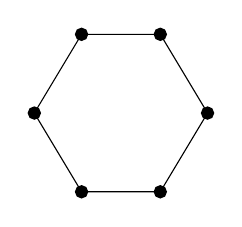
\begin{tikzpicture}
    \tikzstyle{point}=[circle,thick,draw=black,fill=black,inner sep=0pt,minimum width=4pt,minimum height=4pt]
    \node (a)[point] at (0.4,0) {};
    \node (b)[point] at (1,1) {};
    \node (c)[point] at (2,1) {};
    \node (d)[point] at (2.6,0) {};
    \node (e)[point] at (2,-1) {};
    \node (f)[point] at (1,-1) {};
    \draw (a.center) -- (b.center) -- (c.center) -- (d.center) -- (e.center) -- (f.center) -- cycle;
\end{tikzpicture}
}
        \label{fig:simplizialkomplex-1-d}
    }%
    \subfloat[2D Simplizialkomplex (ohne untere Fläche!)]{
        \parbox[c][4cm]{3.5cm}{\centering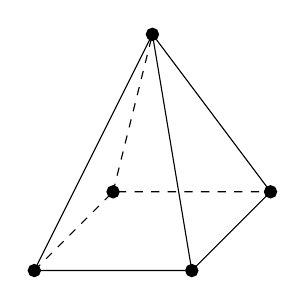
\begin{tikzpicture}
    \tikzstyle{point}=[circle,thick,draw=black,fill=black,inner sep=0pt,minimum width=4pt,minimum height=4pt]
    \node (a)[point] at (0,0) {};
    \node (b)[point] at (2,0) {};
    \node (c)[point] at (3,1) {};
    \node (d)[point] at (1,1) {};
    \node (e)[point] at (1.5,3) {};
    \draw (a.center) -- (b.center) -- (c.center) -- (e.center) -- (b.center);
    \draw (a.center) -- (e.center);
    \draw[dashed] (a.center) -- (d.center) -- (c.center);
    \draw[dashed] (d.center) -- (e.center);
\end{tikzpicture}
}
        \label{fig:simplizialkomplex-2-d}
    }%
    \subfloat[2D Simplizialkomplex]{
        \parbox[c][4cm]{5cm}{\centering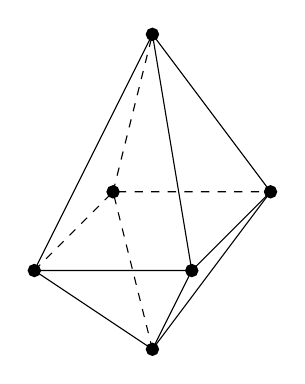
\begin{tikzpicture}
    \tikzstyle{point}=[circle,thick,draw=black,fill=black,inner sep=0pt,minimum width=4pt,minimum height=4pt]
    \node (a)[point] at (0,0) {};
    \node (b)[point] at (2,0) {};
    \node (c)[point] at (3,1) {};
    \node (d)[point] at (1,1) {};
    \node (e)[point] at (1.5,3) {};
    \node (f)[point] at (1.5,-1) {};
    \draw (a.center) -- (b.center) -- (c.center) -- (e.center) -- (b.center);
    \draw (a.center) -- (e.center);
    \draw[dashed] (a.center) -- (d.center) -- (c.center);
    \draw[dashed] (d.center) -- (e.center);

    \draw (a.center) -- (f.center) -- (b.center);
    \draw (f.center) -- (c.center);
    \draw[dashed] (f.center) -- (d.center);
\end{tikzpicture}
}
        \label{fig:simplizialkomplex-2-d-okateder}
    }%

    \subfloat[1D Simplizialkomplex]{
        \parbox[c][4cm]{5cm}{\centering\documentclass[varwidth=true, border=2pt]{standalone}
\usepackage{tikz}

\begin{document}
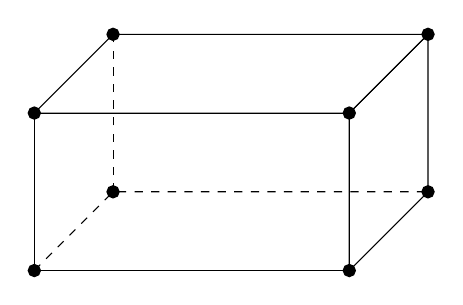
\begin{tikzpicture}
    \tikzstyle{point}=[circle,thick,draw=black,fill=black,inner sep=0pt,minimum width=4pt,minimum height=4pt]
    \node (a)[point] at (0,0) {};
    \node (b)[point] at (4,0) {};
    \node (c)[point] at (5,1) {};
    \node (d)[point] at (1,1) {};
    \node (e)[point] at (0,2) {};
    \node (f)[point] at (4,2) {};
    \node (g)[point] at (5,3) {};
    \node (h)[point] at (1,3) {};
    \draw (a.center) -- (b.center) -- (f.center) -- (e.center) -- cycle;
    \draw (b.center) -- (c.center) -- (g.center) -- (f.center) -- cycle;
    \draw (e.center) -- (f.center) -- (g.center) -- (h.center) -- cycle;
    \draw[dashed] (a.center) -- (d.center) -- (c.center);
    \draw[dashed] (d.center) -- (h.center);
\end{tikzpicture}
\end{document}
}
        \label{fig:simplizialkomplex-cube}
    }%
    \subfloat[2D Simplizialkomplex]{
        \parbox[c][4cm]{5cm}{\centering\documentclass[varwidth=true, border=2pt]{standalone}
\usepackage{tikz}

\begin{document}
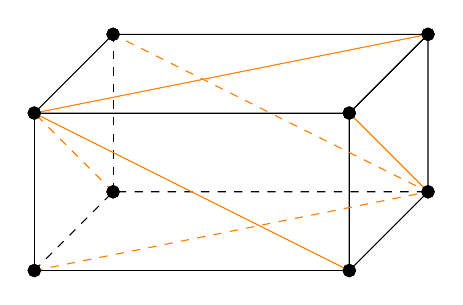
\begin{tikzpicture}
    \tikzstyle{point}=[circle,thick,draw=black,fill=black,inner sep=0pt,minimum width=4pt,minimum height=4pt]
    \node (a)[point] at (0,0) {};
    \node (b)[point] at (4,0) {};
    \node (c)[point] at (5,1) {};
    \node (d)[point] at (1,1) {};
    \node (e)[point] at (0,2) {};
    \node (f)[point] at (4,2) {};
    \node (g)[point] at (5,3) {};
    \node (h)[point] at (1,3) {};
    \draw (a.center) -- (b.center) -- (f.center) -- (e.center) -- cycle;
    \draw (b.center) -- (c.center) -- (g.center) -- (f.center) -- cycle;
    \draw (e.center) -- (f.center) -- (g.center) -- (h.center) -- cycle;
    \draw[dashed] (a.center) -- (d.center) -- (c.center);
    \draw[dashed] (d.center) -- (h.center);

    \draw[orange] (b.center) -- (e.center) -- (g.center);
    \draw[orange,dashed] (a.center) -- (c.center) -- (h.center);
    \draw[orange,dashed] (d.center) -- (e.center);
    \draw[orange] (f.center) -- (c.center);

    \node (a)[point] at (0,0) {};
    \node (b)[point] at (4,0) {};
    \node (c)[point] at (5,1) {};
    \node (d)[point] at (1,1) {};
    \node (e)[point] at (0,2) {};
    \node (f)[point] at (4,2) {};
    \node (g)[point] at (5,3) {};
    \node (h)[point] at (1,3) {};
\end{tikzpicture}
\end{document}
}
        \label{fig:simplizialkomplex-cube-divided}
    }

    \subfloat[$P$ ist kein Teilsimplex, da Eigenschaft \cref{def:simplizialkomplex.ii} verletzt ist]{
        \parbox[c][4cm]{5cm}{\centering\documentclass[varwidth=true, border=2pt]{standalone}
\usepackage{tikz}
\usetikzlibrary{patterns}

\begin{document}
\begin{tikzpicture}
    \tikzstyle{point}=[circle,thick,draw=black,fill=black,inner sep=0pt,minimum width=4pt,minimum height=4pt]
    \node (a)[point] at (0,0) {};
    \node (b)[point] at (3,0) {};
    \node (c)[point] at (2,2) {};

    \begin{scope}[yshift=2cm]
    \node (d)[point] at (1,1) {};
    \node (e)[point] at (0,2) {};
    \node (f)[point] at (4,2) {};
    \end{scope}
    
    \node (p)[point,label={[label distance=0cm]5:$P$}] at (1.5,0.5) {};

    \draw[pattern=north east lines] (a.center) -- (b.center) -- (c.center) -- cycle;
    \draw[pattern=dots] (d.center) -- (e.center) -- (f.center) -- cycle;
    \draw (p.center) -- (d.center);
\end{tikzpicture}
\end{document}
}
        \label{fig:no-simplizialkomplex-triangles}
    }%
    \subfloat[Simplizialkomplex]{
        \parbox[c][4cm]{5cm}{\centering\begin{tikzpicture}
    \tikzstyle{point}=[circle,thick,draw=black,fill=black,inner sep=0pt,minimum width=4pt,minimum height=4pt]
    \node (a)[point] at (0,0) {};
    \node (b)[point] at (3,0) {};
    \node (c)[point] at (2,2) {};

    \begin{scope}[yshift=2cm]
    \node (d)[point] at (1,1) {};
    \node (e)[point] at (0,2) {};
    \node (f)[point] at (4,2) {};
    \end{scope}
    
    \node (p)[point,label={[label distance=0cm]5:$P$}] at (1.5,0.5) {};

    \draw[pattern=north east lines] (a.center) -- (p.center) -- (b.center) -- cycle;
    \draw[pattern=north west lines] (a.center) -- (p.center) -- (c.center) -- cycle;
    \draw[pattern=vertical lines]   (b.center) -- (p.center) -- (c.center) -- cycle;
    \draw[pattern=dots] (d.center) -- (e.center) -- (f.center) -- cycle;
    \draw (p.center) -- (d.center);
\end{tikzpicture}
}
        \label{fig:simplizialkomplex-triangles}
    }%
    \label{fig:simplizialkomplexe}
    \caption{Beispiele für Simplizialkomplexe}
\end{figure}

\begin{definition}\xindex{Abbildung!simpliziale}%
    Seien $K, L$ Simplizialkomplexe. Eine stetige Abbildung
    \[f:|K| \rightarrow |L|\]
    heißt \textbf{simplizial}, wenn für
    jedes $\Delta \in K$ gilt:
    \begin{defenum}
        \item $f(\Delta) \in L$
        \item $f|_{\Delta} : \Delta \rightarrow f(\Delta)$ ist eine
              affine Abbildung.
    \end{defenum}
\end{definition}

\begin{beispiel}[Simpliziale Abbildungen]
    \begin{bspenum}
        \item $\varphi(e_1) := b_1$, $\varphi(e_2) := b_2$\\
              $\varphi$ ist eine eindeutig bestimmte lineare Abbildung

              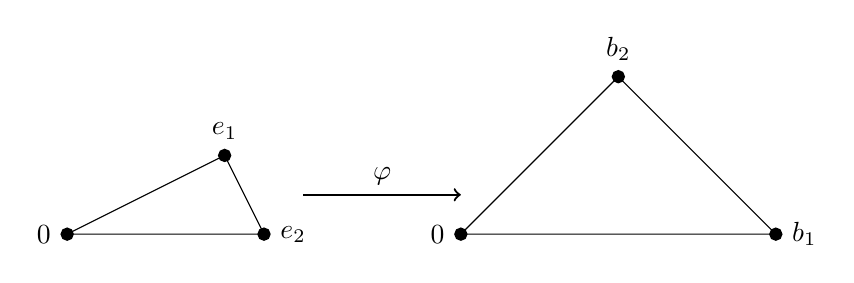
\begin{tikzpicture}
    \tikzstyle{point}=[circle,thick,draw=black,fill=black,inner sep=0pt,minimum width=4pt,minimum height=4pt]

    \node (a)[point,label={[label distance=0cm]180:$0$}] at (0,0) {};
    \node (b)[point,label={[label distance=0cm]0:$e_2$}] at (2.5,0) {};
    \node (c)[point,label={[label distance=0cm]90:$e_1$}] at (2,1) {};

    \begin{scope}[xshift=5cm]
        \node (d)[point,label={[label distance=0cm]180:$0$}] at (0,0) {};
        \node (e)[point,label={[label distance=0cm]0:$b_1$}] at (4,0) {};
        \node (f)[point,label={[label distance=0cm]90:$b_2$}] at (2,2) {};
    \end{scope}

    \draw (a.center) -- (b.center) -- (c.center) -- cycle;
    \draw (d.center) -- (e.center) -- (f.center) -- cycle;

    \draw[thick,->] (3,0.5) -- node[above] {$\varphi$} (5,0.5);
\end{tikzpicture}


        \item Folgende Abbildung $\varphi: \Delta^n \rightarrow \Delta^{n-1}$ 
              ist simplizial:

              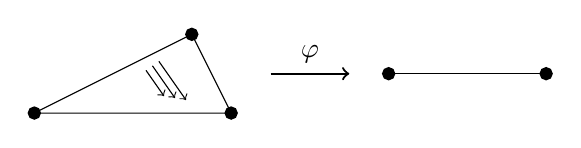
\begin{tikzpicture}
    \tikzstyle{point}=[circle,thick,draw=black,fill=black,inner sep=0pt,minimum width=4pt,minimum height=4pt]

    \node (a)[point] at (0,0) {};
    \node (b)[point] at (2.5,0) {};
    \node (c)[point] at (2,1) {};

    \begin{scope}[xshift=4.5cm, yshift=0.5cm]
        \node (d)[point] at (0,0) {};
        \node (e)[point] at (2,0) {};
    \end{scope}

    \begin{scope}[xshift=1.5cm,yshift=0.6cm,rotate=-55]
    \draw[->] (0,-0.1) -- (0.4,-0.1);
    \draw[->] (0, 0.0) -- (0.5, 0.0);
    \draw[->] (0, 0.1) -- (0.6, 0.1);
    \end{scope}

    \draw (a.center) -- (b.center) -- (c.center) -- cycle;
    \draw (d.center) -- (e.center);

    \draw[thick,->] (3,0.5) -- node[above] {$\varphi$} (4,0.5);
\end{tikzpicture}

        \item Tori können simplizial auf Sphären abgebildet werden:

            \resizebox{0.9\linewidth}{!}{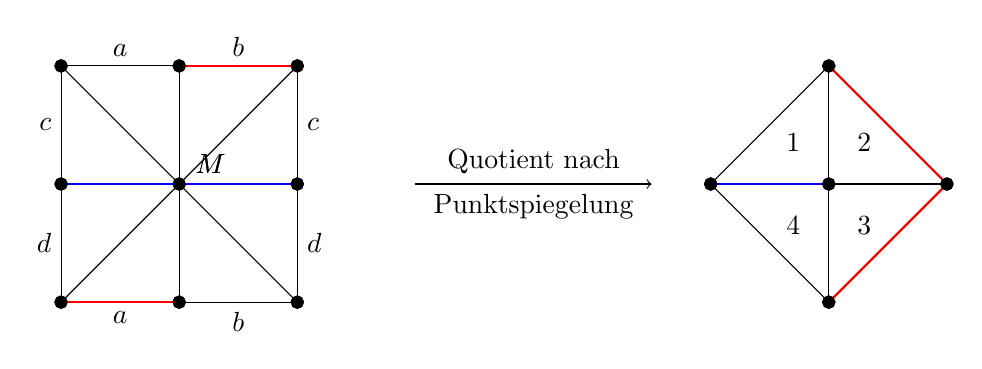
\begin{tikzpicture}[scale=1.5]
    \tikzstyle{point}=[circle,thick,draw=black,fill=black,inner sep=0pt,minimum width=4pt,minimum height=4pt]
    \node (a)[point] at (0,0) {};
    \node (b)[point] at (1,0) {};
    \node (c)[point] at (2,0) {};

    \node (d)[point] at (0,1) {};
    \node (M)[point,label={[label distance=0cm]5:$M$}] at (1,1) {};
    \node (f)[point] at (2,1) {};

    \node (g)[point] at (0,2) {};
    \node (h)[point] at (1,2) {};
    \node (i)[point] at (2,2) {};

    \draw (a.center) -- node[below] {$a$} (b.center);
    \draw (b.center) -- node[below] {$b$} (c.center);
    \draw (g.center) -- node[above] {$a$} (h.center);
    \draw (h.center) -- node[above] {$b$} (i.center);
    \draw (d.center) -- node[left] {$c$} (g.center);
    \draw (d.center) -- node[left] {$d$} (a.center);
    \draw (f.center) -- node[right] {$d$} (c.center);
    \draw (i.center) -- node[right] {$c$} (f.center);

    \draw (a.center) -- (b.center) -- (M.center) -- (d.center) -- cycle;
    \draw (b.center) -- (c.center) -- (f.center) -- (M.center) -- cycle;
    \draw (d.center) -- (M.center) -- (h.center) -- (g.center) -- cycle;
    \draw (M.center) -- (f.center) -- (i.center) -- (h.center) -- cycle;

    \draw[thick, blue] (d.center) -- (M.center) -- (f.center);

    \draw[thick, red] (a.center) -- (b.center);
    \draw[thick, red] (h.center) -- (i.center);

    % Draw again so that lines are below nodes
    \draw (a.center) -- (i.center);
    \draw (c.center) -- (g.center);

    \node (a)[point] at (0,0) {};
    \node (b)[point] at (1,0) {};
    \node (c)[point] at (2,0) {};

    \node (d)[point] at (0,1) {};
    \node (M)[point,label={[label distance=0cm]5:$M$}] at (1,1) {};
    \node (f)[point] at (2,1) {};

    \node (g)[point] at (0,2) {};
    \node (h)[point] at (1,2) {};
    \node (i)[point] at (2,2) {};

    \draw[->] (3,1) -- node[above] {Quotient nach} node[below] {Punktspiegelung} (5,1);

    \begin{scope}[xshift=6.5cm,yshift=1cm]
        \node (w)[point] at (-1,0) {};
        \node (x)[point] at (0,-1) {};
        \node (y)[point] at (1,0) {};
        \node (z)[point] at (0,1) {};
        \node (m)[point] at (0,0) {};

        \node (1) at (-0.3,+0.35) {1};
        \node (2) at (+0.3,+0.35) {2};
        \node (3) at (+0.3,-0.35) {3};
        \node (4) at (-0.3,-0.35) {4};

        \draw (w.center) -- (x.center) -- (y.center) -- (z.center) -- cycle;

        \draw[thick, blue] (w.center) -- (m.center);
        \draw (m.center) -- (y.center);
        \draw (x.center) -- (m.center) -- (z.center);
        \draw[thick, red] (z.center) -- (y.center) -- (x.center);

        % Draw again, as lines should be below points
        \node (w)[point] at (-1,0) {};
        \node (x)[point] at (0,-1) {};
        \node (y)[point] at (1,0) {};
        \node (z)[point] at (0,1) {};
        \node (m)[point] at (0,0) {};
    \end{scope}
\end{tikzpicture}
}
    \end{bspenum}
\end{beispiel}

\begin{definition}\xindex{Eulerzahl}%
    Sei $K$ ein endlicher Simplizialkomplex. Für $n \geq 0$ sei
    $a_n(K)$ die Anzahl der $n$-Simplizes in $K$.

    Dann heißt 
    \[\chi(K) := \sum_{n=0}^{\dim K} (-1)^n a_n(K)\]
    \textbf{Eulerzahl} (oder Euler-Charakteristik\index{Euler-Charakteristik|see{Eulerzahl}})
    von $K$.
\end{definition}

\begin{beispiel}
    \begin{bspenum}
        \item $\chi(\Delta^1) = 2 - 1 = 1$\\
              $\chi(\Delta^2) = 3 - 3 + 1 = 1$\\
              $\chi(\Delta^3) = 4 - 6 + 4 - 1 = 1$
        \item $\chi(\text{Oktaeder-Oberfläche}) = 6 - 12 + 8 = 2$\\
              $\chi(\text{Rand des Tetraeders}) = 2$\\
              $\chi(\text{Ikosaeder}) = 12 - 30 + 20 = 2$
        \item $\chi(\text{Würfel}) = 8 - 12 + 6 = 2$\\
              $\chi(\text{Würfel, unterteilt in Dreiecksflächen}) = 8 - (12 + 6) + (6 \cdot 2) = 2$
    \end{bspenum}
\end{beispiel}

\begin{bemerkung}
    $\chi(\Delta^n) = 1$ für jedes $n \in \mdn_0$
\end{bemerkung}

\begin{beweis}
    $\Delta^n$ ist die konvexe Hülle von $(e_0, \dots, e_n)$ in $\mdr^{n+1}$.
    Jede $(k+1)$-elementige Teilmenge von $\Set{e_0, \dots, e_n}$
    definiert ein $k$-Simplex.\\
    $\Rightarrow a_k(\Delta^n) = \binom{n+1}{k+1}, \;\;\; k = 0, \dots, n$\\
    $\Rightarrow \chi(\Delta^n) = \sum_{k=0}^n (-1)^k \binom{n+1}{k+1}$\\
    $f(x) = (x+1)^{n+1} \overset{\substack{\text{\tiny{Binomischer}}\\\text{\tiny{Lehrsatz}}}}{=} \sum_{k=0}^{n+1} \binom{n+1}{k} x^k$\\
    $\Rightarrow 0 = \sum_{k=0}^{n+1} \binom{n+1}{k} (-1)^k = \chi(\Delta^n) -1$\\
    $\Rightarrow \chi(\Delta^n) = 1 \qed$
\end{beweis}

%%%%%%%%%%%%%%%%%%%%%%%%%%%%%%%%%%%%%%%%%%%%%%%%%%%%%%%%%%%%%%%%%%%%%
% Mitschrieb vom 28.11.2013                                         %
%%%%%%%%%%%%%%%%%%%%%%%%%%%%%%%%%%%%%%%%%%%%%%%%%%%%%%%%%%%%%%%%%%%%%
\begin{definition}%
    \begin{defenum}
        \item Ein 1D-Simplizialkomplex heißt \textbf{Graph}\xindex{Graph}.
        \item Ein Graph, der homöomorph zu $S^1$ ist, heißt \textbf{Kreis}\xindex{Kreis}.
        \item Ein zusammenhängender Graph heißt \textbf{Baum}\xindex{Baum},
              wenn er keinen Kreis enthält.
    \end{defenum}
\end{definition}

\begin{figure}[ht]
    \centering
    \subfloat[Dies wird häufig auch als Multigraph bezeichnet.]{
        \parbox[c][3cm]{4cm}{\centering\documentclass[varwidth=true, border=2pt]{standalone}
\usepackage{tikz}

\begin{document}
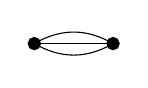
\begin{tikzpicture}
    \tikzstyle{point}=[circle,thick,draw=black,fill=black,inner sep=0pt,minimum width=4pt,minimum height=4pt]
    \node (a)[point] at (0,0) {};
    \node (b)[point] at (1,0) {};
    \path (a.center) edge [bend left]  (b.center);
    \path (a.center) edge              (b.center);
    \path (a.center) edge [bend right] (b.center);
\end{tikzpicture}
\end{document}
}
        \label{fig:topology-graph-simple}
    }%
    \subfloat[Planare Einbettung des Tetraeders]{
        \parbox[c][3cm]{4cm}{\centering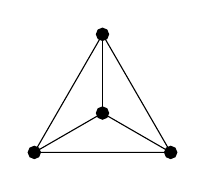
\begin{tikzpicture}
    \tikzstyle{point}=[circle,thick,draw=black,fill=black,inner sep=0pt,minimum width=4pt,minimum height=4pt]
    \node (z)[point] at (0,0) {};
    \node (a)[point] at (90:1cm) {};
    \node (b)[point] at (210:1cm) {};
    \node (c)[point] at (330:1cm) {};
    \path (z.center) edge (a.center);
    \path (z.center) edge (b.center);
    \path (z.center) edge (c.center);
    \draw (a.center) -- (b.center) -- (c.center) -- cycle;
\end{tikzpicture}
}
        \label{fig:topology-graph-tetraeder}
    }

    \subfloat[$K_5$]{
        \parbox[c][3cm]{4cm}{\centering    \newcommand\n{5}
    \begin{tikzpicture}
        \tikzstyle{point}=[circle,thick,draw=black,fill=black,inner sep=0pt,minimum width=4pt,minimum height=4pt]

        \begin{scope}[rotate=17]
        %the multiplication with floats is not possible. Thus I split the loop in two.
        \foreach \number in {1,...,\n}{
            \node[point] (N-\number) at ({\number*(360/\n)}:1.5cm) {};
        }

        \foreach \number in {1,...,\n}{
            \foreach \y in {1,...,\n}{
                \draw (N-\number) -- (N-\y);
            }
        }
        \end{scope}
    \end{tikzpicture}
}
        \label{fig:k-5}
    }%
    \subfloat[$K_{3,3}$]{
        \parbox[c][3cm]{4cm}{\centering\documentclass[varwidth=true, border=2pt]{standalone}
\usepackage{tikz}

\begin{document}
    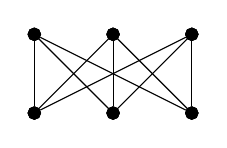
\begin{tikzpicture}
        \tikzstyle{point}=[circle,thick,draw=black,fill=black,inner sep=0pt,minimum width=4pt,minimum height=4pt]

        \foreach \x in {0,1,2}
        \foreach \y in {0,1,2}{
          \node (a)[point] at (\y,0) {};
          \node (b)[point] at (\x,1) {};
            \draw (a) -- (b);
        }
    \end{tikzpicture}
\end{document}
}
        \label{fig:k-3-3}
    }%
    \caption{Beispiele für Graphen}
    \label{fig:graphen-beispiele}
\end{figure}

\begin{bemerkung}
    Für jeden Baum $T$ gilt $\gamma(T) = 1$.
\end{bemerkung}

\begin{beweis}
    Induktion über die Anzahl der Ecken.
\end{beweis}

\begin{bemerkung}
    \begin{bemenum}
        \item Jeder zusammenhängende Graph $\Gamma$ enthält einen
              Teilbaum $T$, der alle Ecken von $\Gamma$ enthält.%
              \footnote{$T$ wird \enquote{Spannbaum} genannt.}
        \item Ist $n = a_1(\Gamma) - a_1(T)$, so ist $\chi(\Gamma) = 1 - n$.
    \end{bemenum}
\end{bemerkung}

\begin{beweis}\leavevmode
    \begin{enumerate}[label=\alph*),ref=\thedefinition.\alph*]
        \item Siehe \enquote{Algorithmus von Kruskal}.
        \item $\begin{aligned}[t]\chi(\Gamma) &= a_0(\Gamma) - a_1(\Gamma)\\
                                        &= a_0(\Gamma) - (n+a_1(T))\\
                                        &= a_0(T) - a_1(T) - n\\
                                        &= \chi(T) - n\\
                                        &= 1-n
              \end{aligned}$
    \end{enumerate}
\end{beweis}

\begin{bemerkung}\label{kor:simplex-unterteilung}
    Sei $\Delta$ ein $n$-Simplex und $x \in \Delta^\circ \subseteq \mdr^n$.
    Sei $K$ der Simplizialkomplex, der aus $\Delta$ durch 
    \enquote{Unterteilung} in $x$ entsteht. Dann ist $\chi(K) = \chi(\Delta) = 1$.
\end{bemerkung}

\begin{figure}[ht]
    \centering
    \subfloat[$K$]{
        \parbox{4cm}{\centering\begin{tikzpicture}
    \tikzstyle{point}=[circle,thick,draw=black,fill=black,inner sep=0pt,minimum width=4pt,minimum height=4pt]
    \node (z)[point] at (0,0) {};
    \node (a)[point] at (90:1cm) {};
    \node (b)[point] at (210:1cm) {};
    \node (c)[point] at (330:1cm) {};
    \path (z.center) edge (a.center);
    \path (z.center) edge (b.center);
    \path (z.center) edge (c.center);
    \draw (a.center) -- (b.center) -- (c.center) -- cycle;

    \draw[pattern=north west lines] (a.center) -- (b.center) -- (z.center) --cycle;
    \draw[pattern=dots] (b.center) -- (c.center) -- (z.center) --cycle;
    \draw[pattern=crosshatch] (a.center) -- (c.center) -- (z.center) --cycle;
\end{tikzpicture}
}
        \label{fig:topology-simplizial-complex-k}
    }%
    \subfloat[$\Delta$, das aus $K$ durch Unterteilung entsteht]{
        \parbox{4cm}{\centering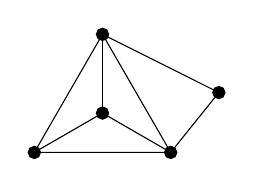
\begin{tikzpicture}
    \tikzstyle{point}=[circle,thick,draw=black,fill=black,inner sep=0pt,minimum width=4pt,minimum height=4pt]
    \node (z)[point] at (0,0) {};
    \node (a)[point] at (90:1cm) {};
    \node (b)[point] at (210:1cm) {};
    \node (c)[point] at (330:1cm) {};
    \node (d)[point] at (10:1.5cm) {};
    \path (z.center) edge (a.center);
    \path (z.center) edge (b.center);
    \path (z.center) edge (c.center);
    \draw (a.center) -- (b.center) -- (c.center) -- cycle;

    \draw (a.center) -- (d.center);
    \draw (c.center) -- (d.center);
\end{tikzpicture}
}
        \label{fig:topology-simplizial-complex-k-division}
    }%
    \caption{Beispiel für \cref{kor:simplex-unterteilung}.}
    \label{fig:simplex-unterteilung-beispiel}
\end{figure}

\begin{beweis}
    $\chi(K) = \chi(\Delta) - \underbrace{\underbrace{(-1)^n}_{n\text{-Simplex}} + \sum_{k=0}^n (-1)^k \binom{n+1}{k}}_{(1+(-1))^{n+1}} = \chi(\Delta) \qed$
\end{beweis}

\begin{satz}[Eulersche Polyederformel]\xindex{Eulersche Polyederformel}%
    Sei $P$ ein konvexes Polyeder in $\mdr^3$, d.~h. $\partial P$ ist
    ein 2-dimensionaler Simplizialkomplex, sodass gilt:
    \[\forall x,y \in \partial P: [x,y] \subseteq P\]

    Dann ist $\chi(\partial P) = 2$.
\end{satz}

\begin{beweis}\leavevmode
    \begin{enumerate}[label=\arabic*)]
        \item Die Aussage ist richtig für den Tetraeder.
        \item \Obda{} sei $0 \in P$ und $P \subseteq \fB_1(0)$. Projeziere
              $\partial P$ von $0$ aus auf $\partial \fB_1(0) = S^2$.
              Erhalte Triangulierung von $S^2$.
        \item Sind $P_1$ und $P_2$ konvexe Polygone und $T_1, T_2$
              die zugehörigen Triangulierungen von $S^2$, so gibt es 
              eine eine Triangulierungen $T$, die sowohl um $T_1$ als
              auch um $T_2$ Verfeinerung ist (vgl. \cref{fig:topology-3}).

              \begin{figure}[htp]
                  \centering
                  \newenvironment{customlegend}[1][]{%
    \begingroup
    % inits/clears the lists (which might be populated from previous
    % axes):
    \csname pgfplots@init@cleared@structures\endcsname
    \pgfplotsset{#1}%
}{%
    % draws the legend:
    \csname pgfplots@createlegend\endcsname
    \endgroup
}%

% makes \addlegendimage available (typically only available within an
% axis environment):
\def\addlegendimage{\csname pgfplots@addlegendimage\endcsname}

%%--------------------------------

% definition to insert numbers
\pgfkeys{/pgfplots/number in legend/.style={%
        /pgfplots/legend image code/.code={%
            \node at (0.295,-0.0225){#1};
        },%
    },
}

\pgfdeclarelayer{background}
\pgfdeclarelayer{foreground}
\pgfsetlayers{background,main,foreground}
\begin{tikzpicture}
    \tkzSetUpPoint[shape=circle,size=10,color=black,fill=black]

    \tkzDefPoints{0/0/A, 2/0/B, 3/0.5/C, 0/3/D, 2/3/E, 3/1.5/F, 2/2/G, 1/1.5/H}

    \begin{pgfonlayer}{foreground}
        %Get intersections
        \tkzInterLL(B,H)(A,C) \tkzGetPoint{I}
        \tkzInterLL(B,F)(A,C) \tkzGetPoint{J}
        \tkzInterLL(A,G)(B,H) \tkzGetPoint{K}
        \tkzInterLL(A,G)(H,F) \tkzGetPoint{L}
        \tkzInterLL(C,G)(B,F) \tkzGetPoint{M}
        \tkzInterLL(C,G)(H,F) \tkzGetPoint{N}
        \tkzInterLL(G,D)(H,E) \tkzGetPoint{O}

        \tkzDrawPoints[color=green,fill=green](A,C,G,D)
        \tkzDrawPoints[color=blue,fill=blue](B,F,E,H)
        \tkzDrawPoints[color=red,fill=red](I,J,K,L,M,N,O)
    \end{pgfonlayer}

    \tkzDrawPolygon[blue,very thick](H,E,F,B)
    \tkzDrawSegment[blue,very thick](H,F)

    \tkzDrawPolygon[green,very thick](A,D,G,C)
    \tkzDrawSegment[green,very thick](A,G)

    \tkzDrawSegments[red,very thick](I,M I,N I,L A,H H,D L,O N,E G,E)

    % \tkzLabelPoint(A){A}
    % \tkzLabelPoint(B){B}
    % \tkzLabelPoint(C){C}
    % \tkzLabelPoint(D){D}
    % \tkzLabelPoint(E){E}
    % \tkzLabelPoint(F){F}
    % \tkzLabelPoint(G){G}
    % \tkzLabelPoint(H){H}
    % \tkzLabelPoint(I){I}
    % \tkzLabelPoint(J){J}
    % \tkzLabelPoint(K){K}
    % \tkzLabelPoint(L){L}
    % \tkzLabelPoint(M){M}
    % \tkzLabelPoint(N){N}
    % \tkzLabelPoint(O){O}

    \begin{customlegend}[
    legend entries={
        $T_1$,
        $T_2$,
        $T$
    },
    legend style={at={(4.5,3.5)},font=\footnotesize}] % <= to define position and font legend
    % the following are the "images" and numbers in the legend
        \addlegendimage{blue,very thick}
        \addlegendimage{green,very thick}
        \addlegendimage{red,very thick}
    \end{customlegend}
\end{tikzpicture}
                  \caption{$T$ ist eine Triangulierung, die für $T_1$ und $T_2$ eine Verfeinerung ist.}
                  \label{fig:topology-3}
              \end{figure}

              Nach \cref{kor:simplex-unterteilung} ist
              $\chi(\partial P_1) = \chi(T_1) = \chi(T) = \chi(T_2) = \chi(\partial P_2) = 2$,
              weil \obda{} $P_2$ ein Tetraeder ist.
    \end{enumerate}
\end{beweis}

\begin{bemerkung}[Der Rand vom Rand ist 0]\label{kor:9.11}
    Sei $K$ ein endlicher Simplizialkomplex mit Knotenmenge $V$
    und $<$ eine Totalordnung auf $V$.

    Sei $A_n$ die Menge der $n$-Simplizes in $K$, d.~h.
    \[A_n(K) := \Set{ \sigma \in K | \dim(\sigma) = n}\;\;\; \text{für } n=0, \dots, d=\dim(K)\]

    und $C_n(K)$ der $\mdr$-Vektorraum mit Basis $A_n(K)$, d.~h.
    \[C_n(K) = \Set{\sum_{\sigma \in A_n(K)} c_\sigma \cdot \sigma | c_\sigma \in \mdr}\]

    Sei $\sigma = \Delta(x_0, \dots, x_n) \in A_n(K)$, sodass 
    $x_0 < x_1 < \dots < x_n$.

    Für $i = 0, \dots, n$ sei $\partial_i \sigma := \Delta(x_0, \dots, \hat{x_i}, \dots, x_n)$
    die $i$-te Seite von $\sigma$ und $d_\sigma = d_n \sigma := \sum_{i=0} (-1)^i \partial_i \sigma \in C_{n-1} (K)$
    und $d_n: C_n(K) \rightarrow C_{n-1}(K)$ die dadurch definierte lineare
    Abbildung.

    Dann gilt: $d_{n-1} \circ d_n = 0$
\end{bemerkung}

\begin{beispiel}
    \begin{figure}[h!]
        \centering
        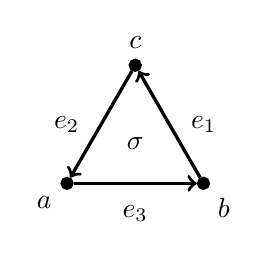
\begin{tikzpicture}
    \tikzstyle{point}=[circle,thick,draw=black,fill=black,inner sep=0pt,minimum width=4pt,minimum height=4pt]
    \node (a)[point,label={[label distance=0cm]210:$a$}] at (210:1cm) {};
    \node (b)[point,label={[label distance=0cm]-45:$b$}] at (330:1cm) {};
    \node (c)[point,label={[label distance=0cm]90:$c$}] at (90:1cm) {};

    \node (sigma) at (0,0) {$\sigma$};

    \draw[->, very thick] (a) edge node[label=below:$e_3$]  {} (b);
    \draw[->, very thick] (b) edge node[label=right:$e_1$]  {} (c);
    \draw[->, very thick] (c) edge node[label=left:$e_2$]  {} (a);
\end{tikzpicture}

        \caption{Simplizialkomplex mit Totalordnung}
    \end{figure}

    Sei $a < b < c$. Dann gilt:

    \begin{align*}
      d_2 \sigma          &= e_1 - e_2 + e_3\\
      d_1(e_1- e_2 + e_3) &= (c - b) - (c-a) + (b - a)\\
                          &= 0
    \end{align*}

    Sei $a<b<c<d$. Dann gilt für Tetraeder:\\
    \begin{align*}
      d_3(\Delta(a,b,c,d)) &= \Delta(b,c,d)-\Delta(a,c,d)+\Delta(a,b,d)-\Delta(a,b,c), \text{wobei:}\\
      d_2(\hphantom{-}\Delta(b,c,d)) &= \hphantom{-}\textcolor{red}{\Delta(c,d)}\textcolor{blue}{-\Delta(b,d)}+\textcolor{green}{\Delta(b,c)}\\
      d_2(-\Delta(a,c,d))  &= \textcolor{red}{-\Delta(c,d)}+\textcolor{black}{\Delta(a,d)}\textcolor{brown}{-\Delta(a,c)}\\
      d_2(\hphantom{-}\Delta(a,b,d)) &= \hphantom{-}\textcolor{blue}{\Delta(b,d)}\textcolor{black}{-\Delta(a,d)}+\textcolor{orange}{\Delta(a,b)}\\
      d_2(-\Delta(a,b,c))  &= \textcolor{green}{-\Delta(b,c)}+\textcolor{brown}{\Delta(a,c)}\textcolor{orange}{-\Delta(a,b)}\\
      \Rightarrow d_2(d_3(\Delta(a,b,c,d))) &=0
    \end{align*}
\end{beispiel}

%%%%%%%%%%%%%%%%%%%%%%%%%%%%%%%%%%%%%%%%%%%%%%%%%%%%%%%%%%%%%%%%%%%%%
% Mitschrieb vom 03.12.2013                                         %
%%%%%%%%%%%%%%%%%%%%%%%%%%%%%%%%%%%%%%%%%%%%%%%%%%%%%%%%%%%%%%%%%%%%%
\begin{beweis}
    Sei $\sigma \in A_n$. Dann gilt:
    \begin{align*}
        d_{n-1}(d_n \sigma) &= d_{n-1} (\sum_{i=0}^n (-1)^i \partial_i \sigma)\\
        &= \sum_{i=0}^n (-1)^i d_{n-1} (\partial_i \sigma)\\
        &= \sum_{i=0}^n (-1)^i \sum_{j=0}^{n-1} \partial_i (\partial_j \sigma) (-1)^j\\
        &= \sum_{\mathclap{0 \leq i \leq j \leq n-1}} (-1)^{i+j} \partial_j (\partial_i (\sigma)) + \sum_{\mathclap{0 \leq j < i \leq n}} (-1)^{i+j} \partial_{i-1} (\partial_j \sigma)\\
        &= 0
    \end{align*}
    weil jeder Summand aus der ersten Summe auch in der zweiten
    Summe vorkommt, aber mit umgekehrten Vorzeichen. $\qed$
\end{beweis}

\begin{definition}%
    Sei $K$ ein Simplizialkomplex, 
    $Z_n := \text{Kern}(d_n) \subseteq C_n$ und 
    $B_n := \text{Bild}(d_{n+1}) \subseteq C_n$.

    \begin{defenum}
        \item $H_n = H_n(K, \mdr) := Z_n / B_n$ heißt $n$-te 
              \textbf{Homologiegruppe}\xindex{Homologiegruppe} von $K$.
        \item $b_n(K) := \dim_{\mdr} H_n$ heißt $n$-te 
              \textbf{Betti-Zahl}\xindex{Betti-Zahl} von $K$.
    \end{defenum}
\end{definition}

\begin{bemerkung}
    Nach \cref{kor:9.11} ist $B_n \subseteq Z_n$, denn
    $d_{n+1}(C) \in \text{Kern}(d_n)$ für $C \in C_{n+1}$.
\end{bemerkung}

\begin{minipage}{\textwidth}%don't break this theorem!
\begin{satz}
    Für jeden endlichen Simplizialkomplex $K$ der Dimension $d$ gilt:

    \[\sum_{k=0}^d (-1)^k b_k (K) = \sum_{k=0}^d (-1)^k a_k(K) = \chi(K) \]
\end{satz}
\end{minipage}

\begin{bemerkung}
    Es gilt \underline{nicht} $a_k = b_k\;\forall k \in \mdn_0$.
\end{bemerkung}

\begin{beweis}\leavevmode
    \begin{itemize}
        \item Dimensionsformel für $d_n$: $a_n = \dim Z_n + \dim B_{n-1}$ für $n \geq 1$
        \item Dimensionsformel für $Z_n \rightarrow H_n = Z_n / B_n: \dim Z_n = b_n + \dim B_n$
        \item $\dim Z_d = b_d$, da $\dim Z_d = b_d + \dim B_d$, wobei $\dim B_d = 0$, da $a_{d+1} = 0$
        \item $a_0 - \dim B_0 = b_0$, da $a_0 - \dim B_0 = a_0 - \dim Z_0 + b_0$ und $a_0 = \dim Z_0$, weil
              $a{-1} = 0$
    \end{itemize}

    \begin{align*}
        \Rightarrow \sum_{k=0}^d (-1)^k a_k &= a_0 + \sum_{k=1}^d (-1)^k (\dim Z_k + \dim B_{k-1})\\
        &= a_0 + \sum_{k=1}^d (-1)^k \dim Z_k + \sum_{k=0}^{d-1} (-1)^{k+1}  \dim B_{k}\\
        &= a_0 + \sum_{k=1}^d (-1)^k \dim Z_k - \sum_{k=0}^{d-1} (-1)^k  \dim B_{k}\\
        &= a_0 + \sum_{k=1}^{d-1} (-1)^k b_k + (-1)^d  \underbrace{\dim Z_d}_{= b_d} - \dim B_0\\
        &= b_0 + \sum_{k=1}^{d-1} (-1)^k b_k + (-1)^d b_d\\
        &= \sum_{k=0}^d (-1)^k b_k
    \end{align*}
\end{beweis}

% \section{Retraktionen}
% \begin{definition}%
%     Sei $X$ ein topologischer Raum, $A \subseteq X$, $r: X \rightarrow A$ eine stetige Abbildung
%     und $\iota: A \hookrightarrow X$ die Inklusionsabbildung.

%     \begin{defenum}
%         \item $r$ heißt \textbf{Retraktion}\xindex{Retraktion}, wenn $r|_A = \id_A$ ist.
%         \item $A$ heißt \textbf{Deformationsretrakt}\xindex{Deformationsretrakt}, wenn es eine Retraktion $r$
%               auf $A$ mit $\iota  \circ r \sim \id_X$ gibt.
%     \end{defenum}
% \end{definition}

% \begin{bemerkung}
% Übungsblatt 7 + 8
% \end{bemerkung}

% Die Übungsaufgaben sollen ganz am Ende des Kapitels sein.
\clearpage
\section*{Übungsaufgaben}
\addcontentsline{toc}{section}{Übungsaufgaben}

\begin{aufgabe}[Zusammenhang]\label{ub4:aufg1}
    \begin{enumerate}[label=(\alph*)]
        \item Beweisen Sie, dass eine topologische Mannigfaltigkeit
              genau dann wegzusammenhängend ist, wenn sie zusammenhängend
              ist
        \item Betrachten Sie nun wie in \cref{bsp:mannigfaltigkeit8}
              den Raum $X:= (\mdr \setminus \Set{0}) \cup \Set{0_1, 0_2}$
              versehen mit der dort definierten Topologie. Ist $X$
              wegzusammenhängend?
    \end{enumerate}
\end{aufgabe}

